% ===================================================================
%  The OpenTex example paper
%  Read it side by side with the PDF: every section explains the
%  LaTeX that produced it. Change anything, then press Compile
%  (Ctrl/Cmd+Enter) to see what happens.
% ===================================================================

% The document class sets the overall look. "article" is the usual
% choice for papers; journals often give you their own class.
\documentclass[11pt]{article}

% Packages add features. Each one is loaded with \usepackage.
\usepackage[margin=1in]{geometry} % page margins
\usepackage{amsmath}              % better equations
\usepackage{graphicx}             % pictures: \includegraphics
\usepackage{booktabs}             % nicer tables: \toprule, \midrule
\usepackage[hidelinks]{hyperref}  % clickable references and links

% Everything before \begin{document} is the "preamble": settings only.
\title{An Example Paper Written in \LaTeX}
\author{Your Name\\Your Institution}
\date{\today}

\begin{document}

\maketitle

% Long papers are easier to work on in pieces. \input{...} pastes in
% another file, so each section can live in its own file.
% !TEX root = ../main.tex
% The line above tells OpenTex (and other editors) which file to
% compile when you press Compile while this file is open.

\begin{abstract}
This short paper shows how to write a scientific paper in \LaTeX{} using OpenTex.
Each section explains the commands used to produce it, so you can learn by reading the source next to the PDF.
By the end you will know how to write text, cite references, add figures, tables and equations, and refer to them by number.
\end{abstract}

% !TEX root = ../main.tex

\section{Introduction}
\label{sec:intro}

In \LaTeX{} each sentence gets a new line.
They will render together normally in the PDF.
Putting every sentence on its own line keeps the source easy to edit, and makes it easy to see what a collaborator changed.

Paragraphs get a blank line in between.
A single line break is just a space; it takes an empty line to start a new paragraph, like this one.

Citations are done like this~\cite{Houston1998}.
The key inside the braces (\texttt{Houston1998}) matches an entry in \texttt{refs.bib}, and \LaTeX{} turns it into a number and adds the reference to the list at the end.
You can cite several works at once~\cite{Knuth1984, Lamport1994}.
In OpenTex, type \verb|\cite{| and a list of your references pops up.
To bring in references from EndNote, Zotero or Mendeley, use \textbf{File $\rightarrow$ Import References}.

You can make text \emph{emphasized}, \textbf{bold}, or \texttt{typewriter}.
Some characters have special meanings in \LaTeX{} and need a backslash to print them: \%, \$, \&, \#, \_.
A plain \% starts a comment, which never appears in the PDF.
% Like this line. Comments are handy for notes to yourself.

You can insert a figure like the one in Section~\ref{sec:results}, and refer to it later by number: see Figure~\ref{fig:example}.
The number is filled in automatically, so it stays correct when you add or move figures.
The same works for sections (Section~\ref{sec:methods}), tables (Table~\ref{tab:samples}) and equations (Equation~\ref{eq:model}).
The \verb|~| is a space that never breaks, so ``Figure'' and its number stay on the same line.

Lists are made like this:
\begin{itemize}
  \item each item starts with \verb|\item|,
  \item use \texttt{enumerate} instead of \texttt{itemize} for a numbered list,
  \item and lists can be nested.
\end{itemize}

% !TEX root = ../main.tex

\section{Methods}
\label{sec:methods}

Inline math goes between dollar signs, like $E = mc^2$ or $\alpha_i \leq \beta^2$.
Subscripts use \verb|_| and superscripts use \verb|^|; put several characters in braces, as in $x_{\mathrm{max}}$.

A numbered equation uses the \texttt{equation} environment:
\begin{equation}
  y(t) = A \, e^{-t/\tau} \cos(\omega t + \phi)
  \label{eq:model}
\end{equation}
where $A$ is the amplitude, $\tau$ the decay time and $\omega$ the angular frequency.
The \verb|\label| inside lets you write Equation~\ref{eq:model} anywhere in the paper.

Several aligned lines use \texttt{align}; the \verb|&| marks where lines line up and \verb|\\| ends a line:
\begin{align}
  \nabla \cdot \mathbf{E} &= \frac{\rho}{\varepsilon_0} \\
  \nabla \times \mathbf{B} &= \mu_0 \mathbf{J} + \mu_0 \varepsilon_0 \frac{\partial \mathbf{E}}{\partial t}
\end{align}

Comments in OpenTex work like comments in Word: select text, click \textbf{+ Comment}, and a collaborator can reply or resolve it.
They are kept in a separate file in the project folder (\texttt{comments.opentex.json}), so they never clutter the text or appear in the PDF.

% !TEX root = ../main.tex

\section{Results}
\label{sec:results}

Figure~\ref{fig:example} shows the measured signal together with the model of Equation~\ref{eq:model}.

% A figure "floats": LaTeX places it where it fits best, near here.
% [tb] means "top or bottom of a page". The picture file lives in the
% figures/ folder; drag your own images into the project and change
% the file name to use them.
\begin{figure}[tb]
  \centering
  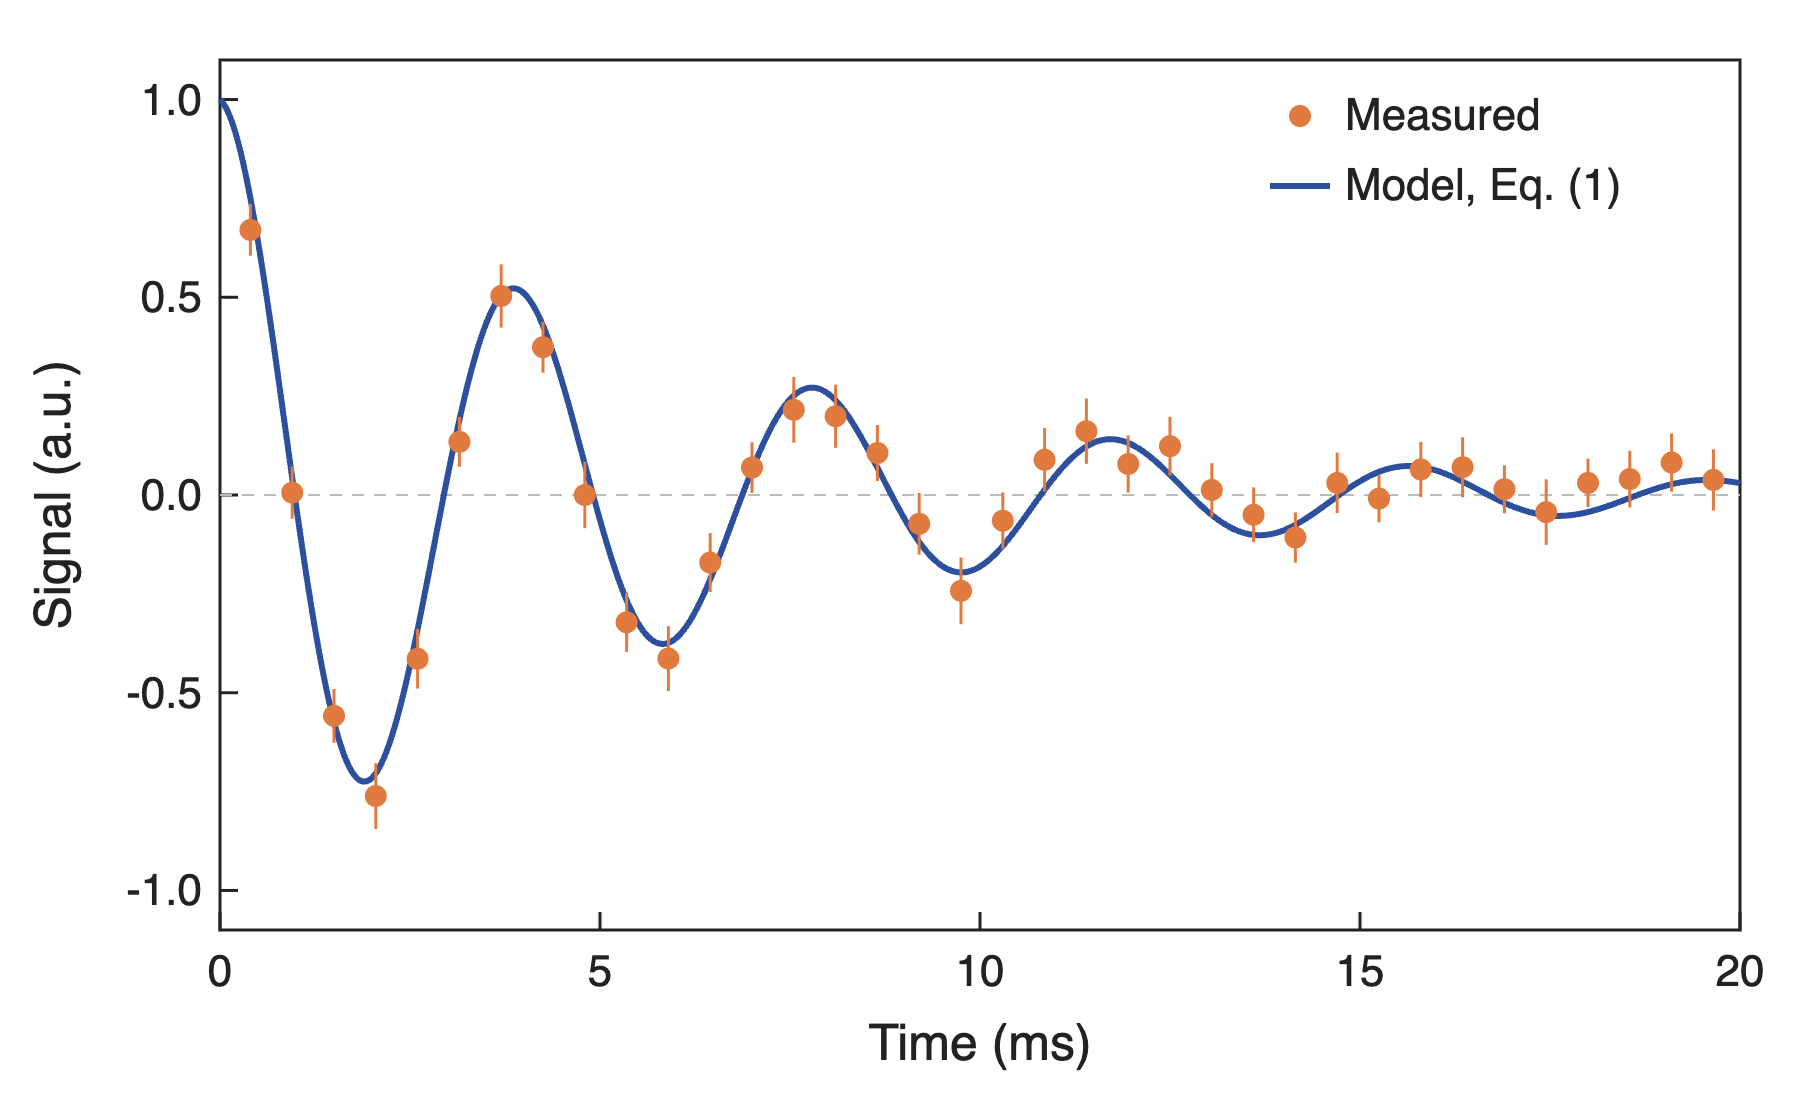
\includegraphics[width=0.75\linewidth]{figures/example-plot.png}
  \caption{Measured signal (points) and the damped-oscillation model of Equation~\ref{eq:model} (line). The caption goes under the picture.}
  \label{fig:example}
\end{figure}

Tables are built from rows: \verb|&| separates columns and \verb|\\| ends a row.
Table~\ref{tab:samples} lists the samples.

\begin{table}[tb]
  \centering
  \caption{Samples used in this study. Table captions usually go above the table.}
  \label{tab:samples}
  \begin{tabular}{lcc}
    \toprule
    Sample & Thickness (nm) & Decay time $\tau$ (ms) \\
    \midrule
    A & 12 & 3.1 \\
    B & 25 & 4.7 \\
    C & 40 & 6.2 \\
    \bottomrule
  \end{tabular}
\end{table}

Double-click anywhere in the PDF and OpenTex jumps to the matching line here.
Press Ctrl/Cmd+J in the source to jump the other way.

% !TEX root = ../main.tex

\section{Conclusions}
\label{sec:conclusions}

You have seen the pieces that make up most scientific papers: sections, citations, figures, tables, equations and cross-references.
A few more tips for working in OpenTex:
\begin{enumerate}
  \item Press Ctrl/Cmd+Enter to compile. Errors appear in a list under the editor; click one to jump to the line.
  \item Focus mode (Ctrl/Cmd+Shift+F) hides everything except the text you are writing.
  \item To start your own paper, use \textbf{File $\rightarrow$ New Project}, or bring in an existing one with \textbf{File $\rightarrow$ Import Word Document}.
  \item Share the whole project folder with collaborators by email, Dropbox or git. Everything, including comments, is in plain text files.
\end{enumerate}

Happy writing!


% The bibliography. \cite{...} commands in the text decide which
% entries from refs.bib appear here. The style controls the format.
\bibliographystyle{plain}
\bibliography{refs}

\end{document}
